\documentclass{article}
\usepackage[utf8]{inputenc}
\usepackage[spanish]{babel}
\usepackage{listings}
\usepackage{subfigure}
\usepackage{graphicx}
\usepackage{url}
\usepackage{multirow}
\usepackage{color}
\usepackage{booktabs}
\usepackage{float}
\usepackage{hyperref}
\usepackage[margin=3cm,twoside]{geometry} 
\setlength{\parindent}{0pt}
\setlength{\parskip}{1em}


\definecolor{mygreen}{rgb}{0,0.6,0}
\definecolor{mygray}{rgb}{0.5,0.5,0.5}
\definecolor{mymauve}{rgb}{0.58,0,0.82}
\lstset{ 
  backgroundcolor=\color{white},   % choose the background color; you must add \usepackage{color} or \usepackage{xcolor}; should come as last argument
  basicstyle=\footnotesize,        % the size of the fonts that are used for the code
  breakatwhitespace=false,         % sets if automatic breaks should only happen at whitespace
  breaklines=true,                 % sets automatic line breaking
  captionpos=b,                    % sets the caption-position to bottom
  commentstyle=\color{mygreen},    % comment style
  deletekeywords={...},            % if you want to delete keywords from the given language
  escapeinside={\%}{)},          % if you want to add LaTeX within your code
  extendedchars=true,              % lets you use non-ASCII characters; for 8-bits encodings only, does not work with UTF-8
  firstnumber=1,                % start line enumeration with line 1000
  frame=single,	                   % adds a frame around the code
  keepspaces=true,                 % keeps spaces in text, useful for keeping indentation of code (possibly needs columns=flexible)
  keywordstyle=\color{blue},       % keyword style
  language=Octave,                 % the language of the code
  morekeywords={*,...},            % if you want to add more keywords to the set
  numbers=left,                    % where to put the line-numbers; possible values are (none, left, right)
  numbersep=5pt,                   % how far the line-numbers are from the code
  numberstyle=\tiny\color{mygray}, % the style that is used for the line-numbers
  rulecolor=\color{black},         % if not set, the frame-color may be changed on line-breaks within not-black text (e.g. comments (green here))
  showspaces=false,                % show spaces everywhere adding particular underscores; it overrides 'showstringspaces'
  showstringspaces=false,          % underline spaces within strings only
  showtabs=false,                  % show tabs within strings adding particular underscores
  stepnumber=1,                    % the step between two line-numbers. If it's 1, each line will be numbered
  stringstyle=\color{mymauve},     % string literal style
  tabsize=2,	                   % sets default tabsize to 2 spaces
  title=\lstname                  % show the filename of files included with \lstinputlisting; also try caption instead of title
}
\usepackage{etoolbox}
\makeatletter
\providecommand{\subtitle}[1]{% add subtitle to \maketitle
  \apptocmd{\@title}{\par {\large #1 \par}}{}{}
}
\makeatother
\title{Tarea 1 de Modelos Probabilistas Aplicados}
\subtitle{Sector Construcción}

\author{5271}
\date{\today}

\begin{document}

\maketitle

\section{Origen de los datos}

Los datos utilizados en este trabajo fueros obtenidos en el sitio \href{https://www.inegi.org.mx/default.html}{https://www.inegi.org.mx} que pertenece al Instituto Nacional de Estadística y Geografía (INEGI). Se escogió el apartado Construcción donde se muestra información sobre los principales resultados de las Empresas Constructoras, comprende unidades económicas dedicadas principalmente a la edificación; a la construcción de obras de ingeniería civil y a la realización de trabajos especializados de construcción. De este apartado se descargó el tabulado (Valor de producción generado por las empresas constructoras según el tipo de obra) en formato \textit{csv}. En el cuadro \ref{tab:frac} de la página \pageref{tab:frac} se muestra un fragmento de los datos descargados. 

% Table generated by Excel2LaTeX from sheet 'Hoja1'
\begin{table}[H]
  \centering
  \caption{Fragmento del tabulado utilizado}
    \begin{tabular}{lrrrrrrrr}
    \toprule
    \multicolumn{1}{c}{\textbf{Periodo}} & \multicolumn{1}{c}{\textbf{Año}} & \multicolumn{1}{c}{\textbf{Total}} & \multicolumn{1}{c}{\textbf{Edific}} & \multicolumn{1}{c}{\textbf{Agua\_R\_S}} & \multicolumn{1}{c}{\textbf{Elect\_C}} & \multicolumn{1}{c}{\textbf{Transp}} & \multicolumn{1}{c}{\textbf{Petr\_p}} & \multicolumn{1}{c}{\textbf{Otras\_C}} \\
    \midrule
    Enero & 2006  & 23649637 & 11562266 & 1527733 & 1062658 & 5237209 & 2698498 & 1561273 \\
    Febrero & 2006  & 23186956 & 11513255 & 1518386 & 808459 & 4901882 & 2931457 & 1513517 \\
    Enero & 2007  & 27801512 & 13848554 & 1314745 & 1011836 & 6078270 & 3554327 & 1993780 \\
    Febrero & 2007  & 27019544 & 13948606 & 949590 & 955818 & 6012856 & 3197691 & 1954983 \\
    Enero & 2020  & 36031814 & 17703639 & 1363041 & 2418338 & 7684282 & 2265532 & 4596982 \\
    Febrero & 2020  & 36626861 & 18064797 & 1186512 & 2189154 & 8031054 & 2539702 & 4615642 \\
    \bottomrule
    \end{tabular}%
  \label{tab:frac}%
\end{table}%

\section{Análisis y tratamiento de los datos}

 Para el análisis de los datos del Valor de producción generado por las empresas constructoras según el tipo de obra, se tiene en cuenta que poseen una frecuencia de ocurrencia mensual, en el periodo comprendido entre los años 2006 y 2020. Por lo que se tratan los mismos como una serie de tiempo. El análisis será realizado en el programa R versión 4.0.2 \cite{r} en el entorno de desarrollo Rstudio \cite{rstudio}. Para llevar al formato de serie de tiempo se realizó el código \ref{cod:1} de la página \pageref{cod:1}.
\begin{center}
\lstinputlisting[language=R, firstline=11, lastline=14]{Series.R}
\label{cod:1}
\end{center}
 \subsection{Análisis}
En el cuadro \ref{tab:sumario} de la página \pageref{tab:sumario} se muestra un resumen de los resultados de varias funciones de ajuste de modelos aplicadas a los datos, Aunque la misma es bastante informativa, pero no tan amigable como una representación gráfica. Por lo anterior es conveniente utilizar el diagrama de caja y bigotes para una mejor comprensión de la información. En la figura \ref{fig:sumario} de la página \pageref{fig:sumario} se muestra la relación entre el valor en miles de pesos corrientes y el tipo de obra.
% Table generated by Excel2LaTeX from sheet 'Sumario'
\begin{table}[H]
  \centering
  \caption{resumen de varias funciones de ajuste de modelos aplicadas}
    \begin{tabular}{lrrrrrr}
    \toprule
          & \multicolumn{1}{l}{\textbf{     Edific               }} & \multicolumn{1}{l}{\textbf{Agua\_R\_S   }} & \multicolumn{1}{l}{\textbf{Elect\_C       }} & \multicolumn{1}{l}{\textbf{Transp       }} & \multicolumn{1}{l}{\textbf{Petr\_p       }} & \multicolumn{1}{l}{\textbf{Otras\_C       }} \\
    \midrule
    \textbf{Min.} & 11513255 & 868901 & 769529 & 4901882 & 1717099 & 1277653 \\
    \textbf{ 1st Qu.} & 14262184 & 1400904 & 1545408 & 7684372 & 2594559 & 2018676 \\
    \textbf{Mediana} & 15600868 & 1596256 & 2267046 & 8712373 & 3007558 & 3458974 \\
    \textbf{Media} & 16013749 & 1606719 & 2280334 & 8453855 & 3122855 & 3351165 \\
    \textbf{ 3rd Qu.} & 17527312 & 1757474 & 2954560 & 9544727 & 3557916 & 4343621 \\
    \textbf{ Max.} & 22055350 & 2517616 & 5320331 & 1.1E+07 & 6061249 & 7027813 \\
    \bottomrule
    \end{tabular}%
  \label{tab:sumario}%
 \vspace{-0.5cm}
\end{table}%
\begin{center}
\begin{figure}[H]
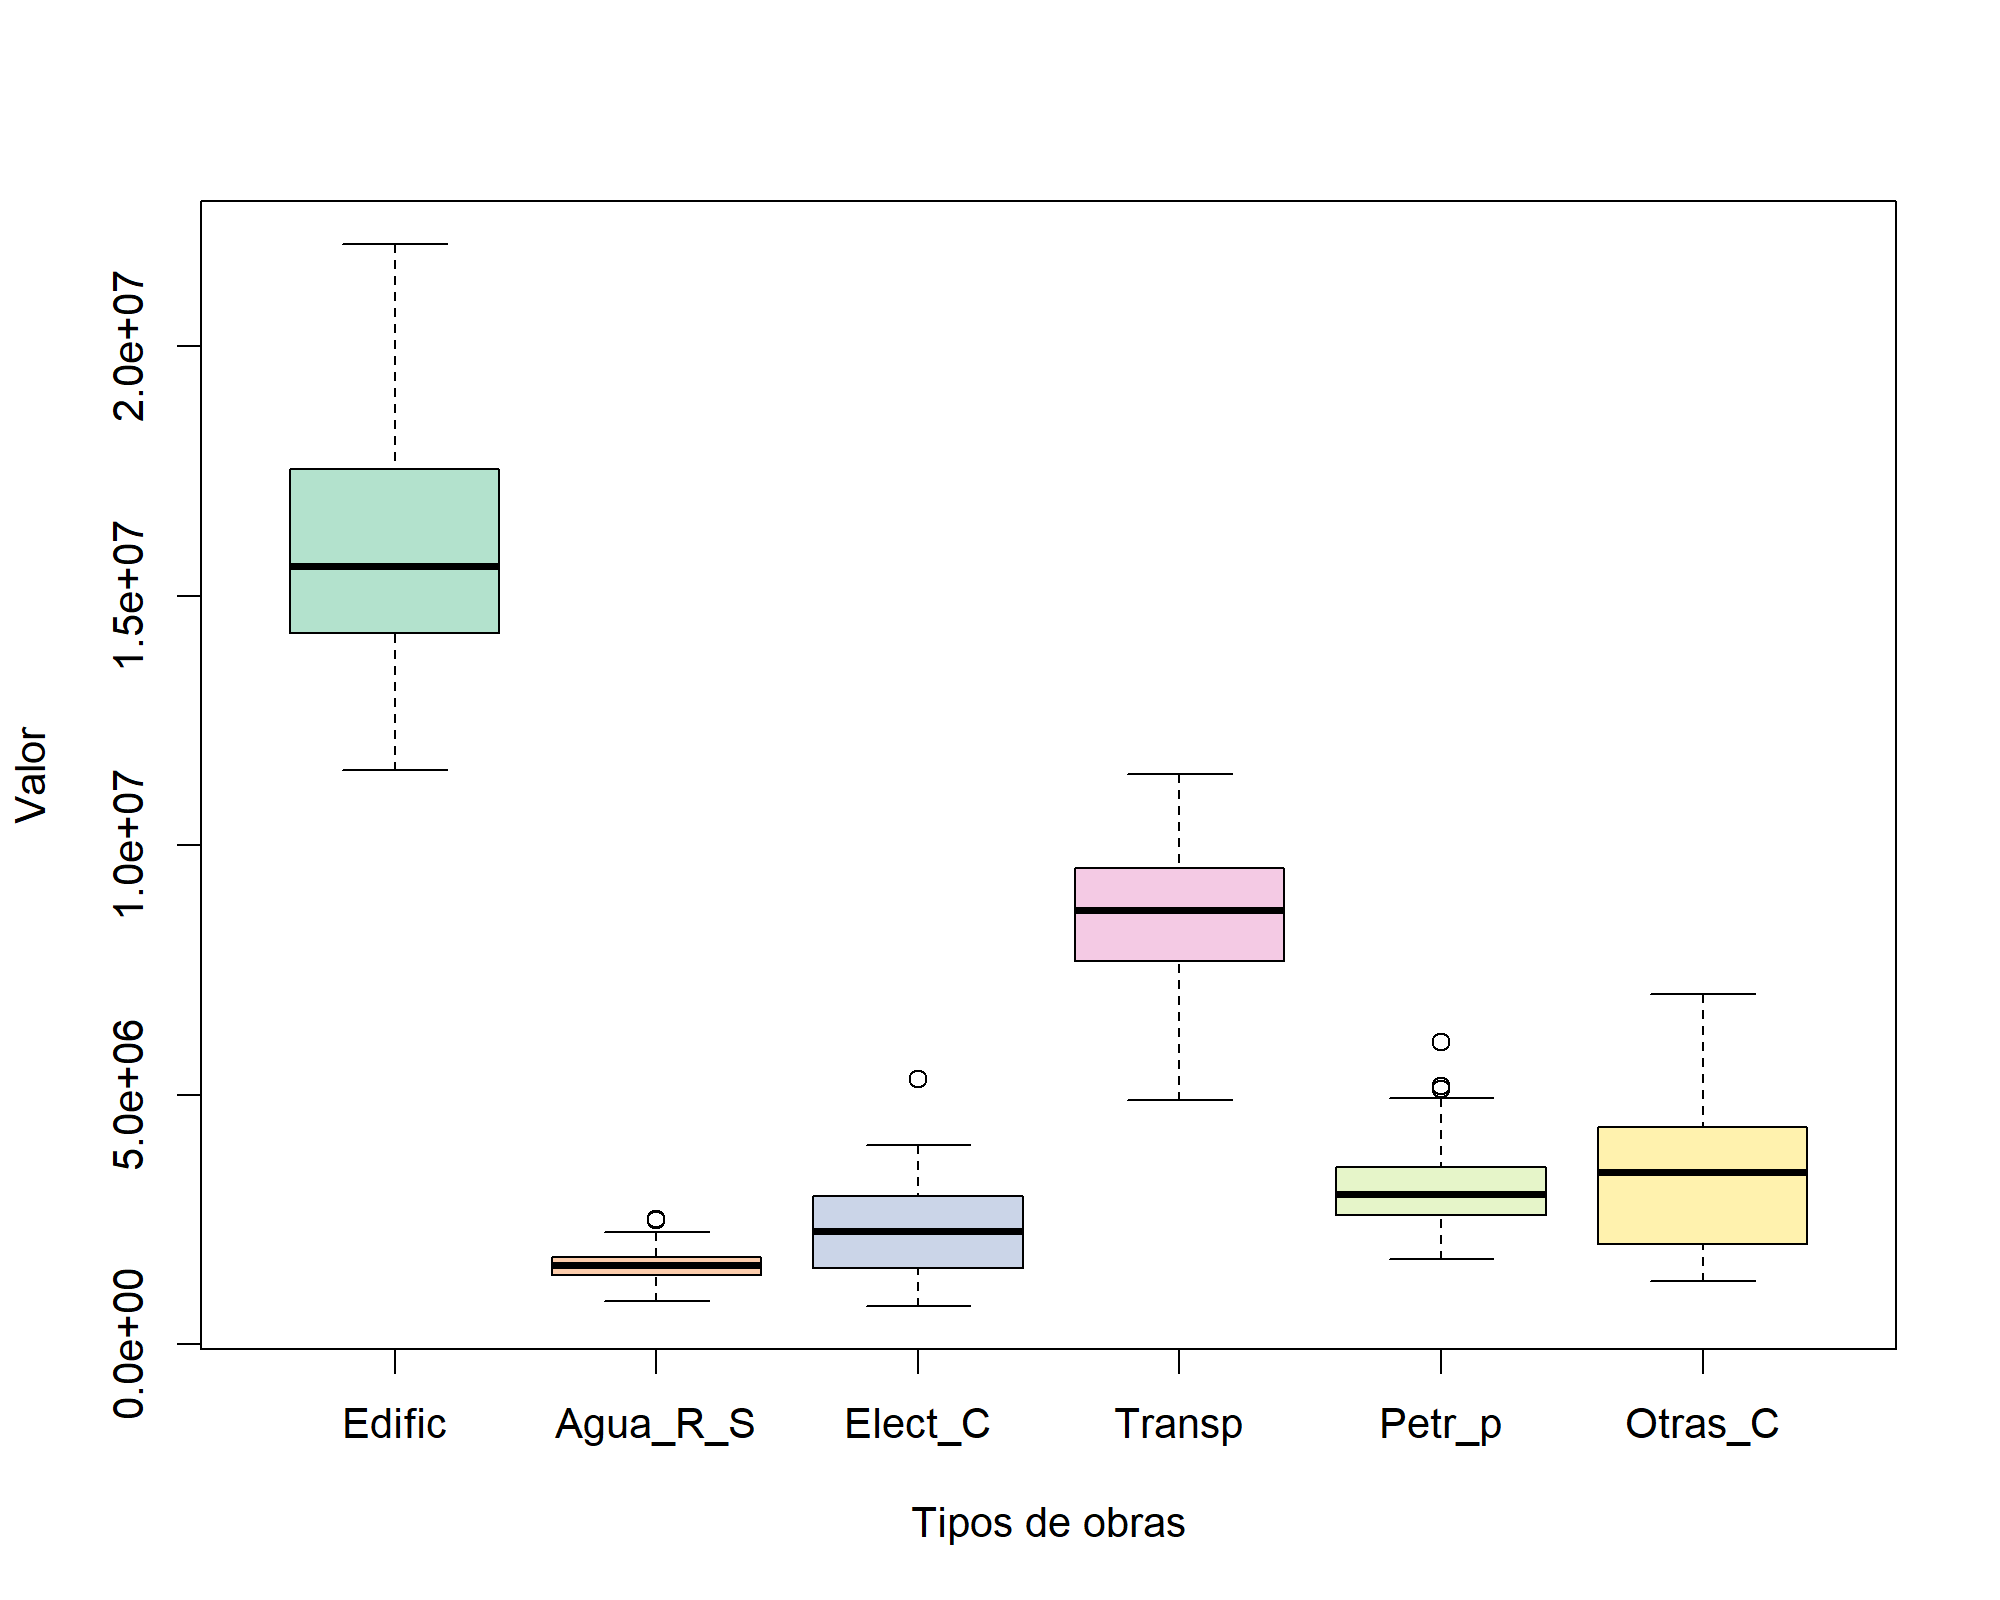
\includegraphics[scale=0.8]{boxplot.png}
\caption{Diagrama de caja y bigotes que relaciona el valor en miles de pesos corrientes con los tipos de obras.}
\label{fig:sumario}
\end{figure}
\end{center}

En el diagrama de caja y bigotes de la figura \ref{fig:sumario}, se puede observar la diferencia entre los valores de los diferentes tipos de obras, además muestra que el tipo de obra Edificaciones es la de mayor valor de producción. Así como las de menor valor son la de Agua, riego y saneamiento y Electricidad y comunicaciones. Lo mismo se puede ver en la figura \ref{fig:serie} de la página \pageref{fig:serie}, donde se muestra una gráfica de secuencia que nos describe el comportamiento del valor de los diferentes tipos de obras a lo largo del tiempo. En la misma refleja que las obras en el sector Petróleo y petroquímica a partir de los años 2016 y 2017 tienen un menor valor que Electricidad y comunicaciones.

\begin{center}
\begin{figure}[H]
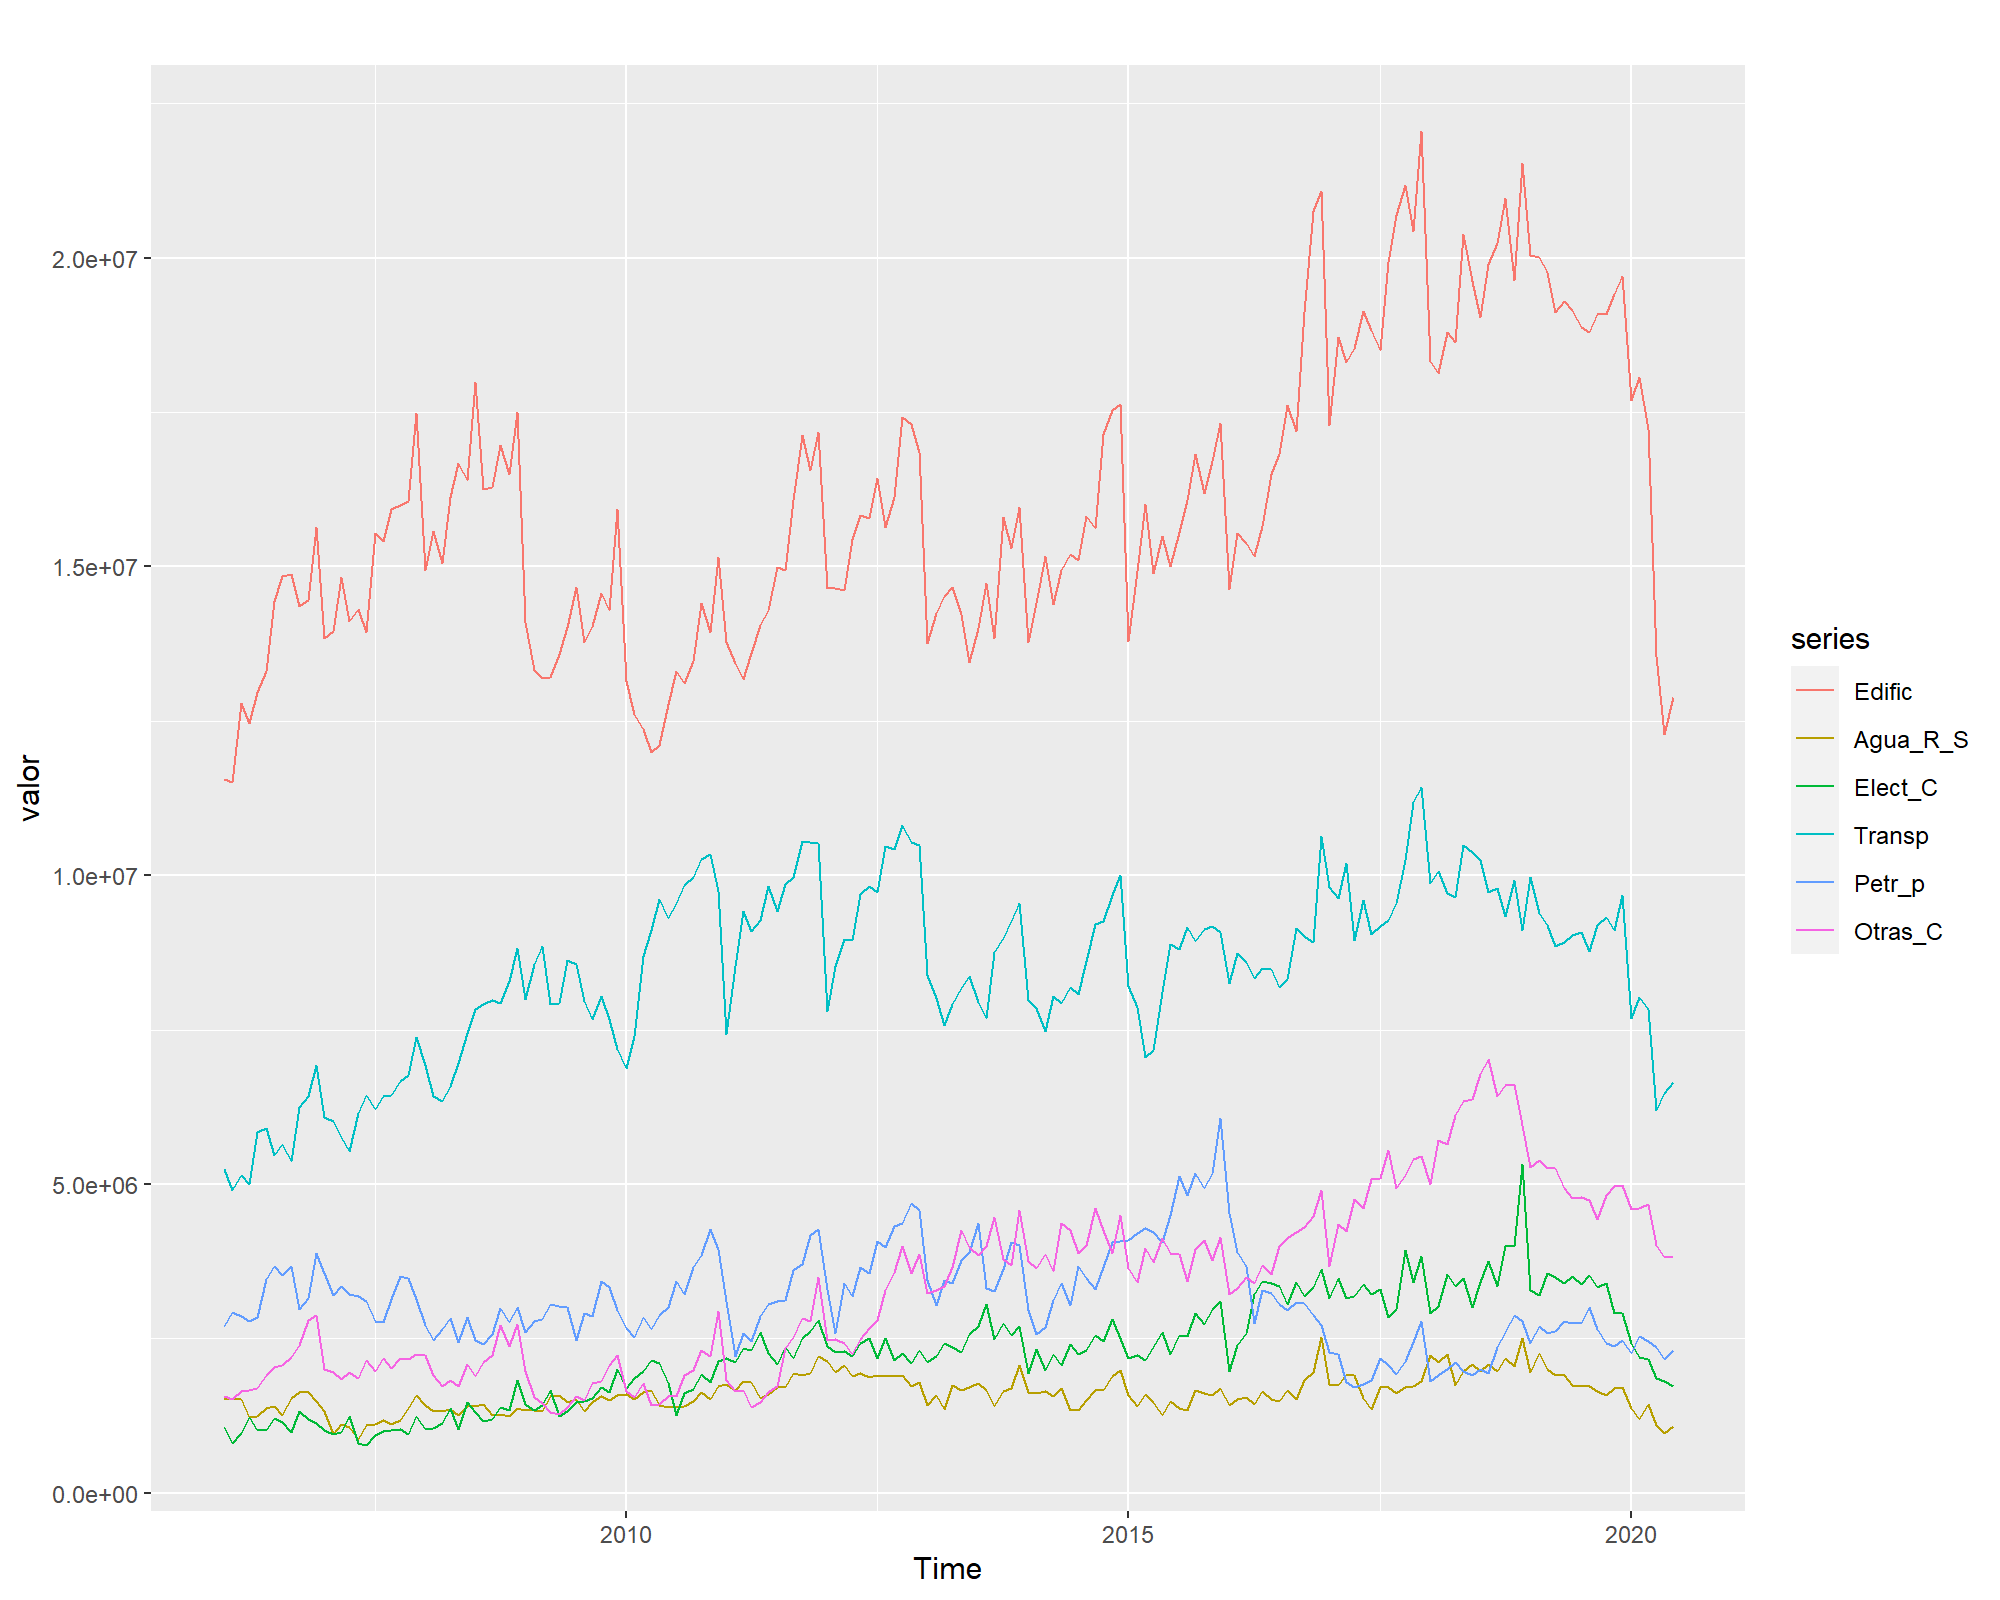
\includegraphics[scale=0.65]{series.png}
\caption{Diagrama de secuencia  que muestra el comportamiento del valor de producción por tipo de obras a lo largo del tiempo.}
\label{fig:serie}
\end{figure}
\end{center}
\newpage
Las figuras \ref{fig:fig1}, \ref{fig:fig2}, \ref{fig:fig3} \ref{fig:fig4}, \ref{fig:fig5}, \ref{fig:fig6} de las paginas \pageref{fig:fig1}, \pageref{fig:fig2}, \pageref{fig:fig3}, \pageref{fig:fig4}, \pageref{fig:fig5}, \pageref{fig:fig6} respectivamente, muestran los valores de producción de cada uno de los tipos de obra por meses. De la interpretación de estos diagramas se pueden inferir que los meses donde mayor valor se reporto fueron octubre, noviembre y diciembre de cada año.  
\begin{center}
\begin{figure}[H]
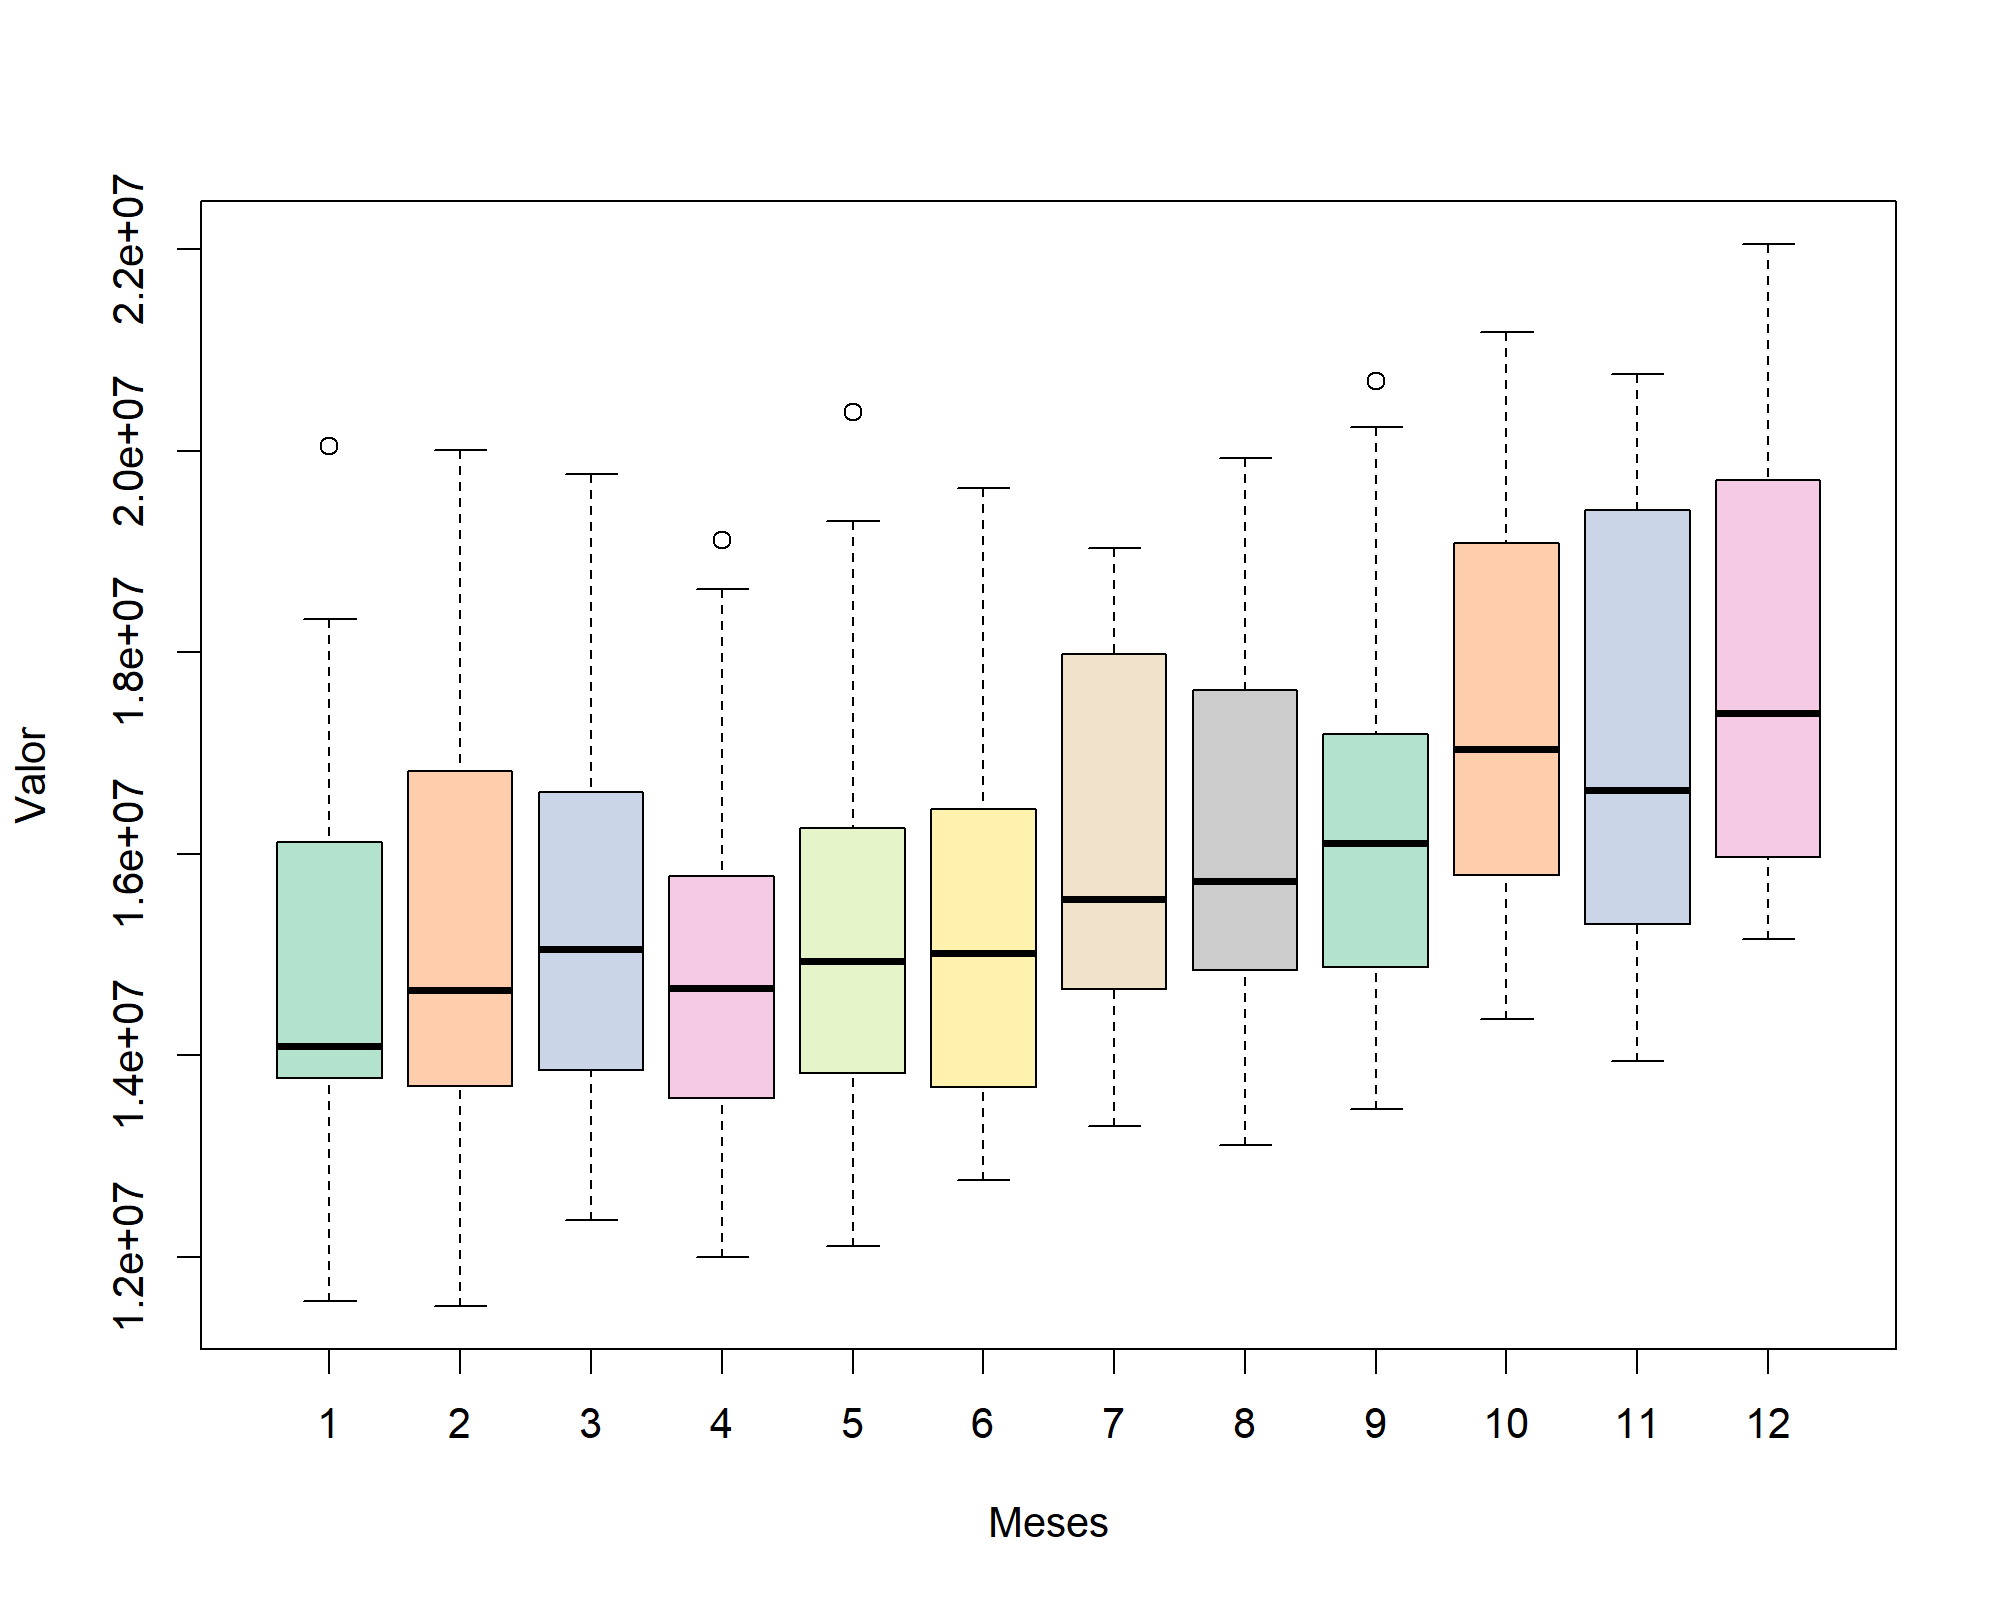
\includegraphics[scale=0.8]{boxplot1.png}
\caption{Diagrama de caja y bigotes del valor de producción del tipo de obra Edificación por meses.}
\label{fig:fig1}
\end{figure}
\end{center}

\begin{center}
\begin{figure}[H]
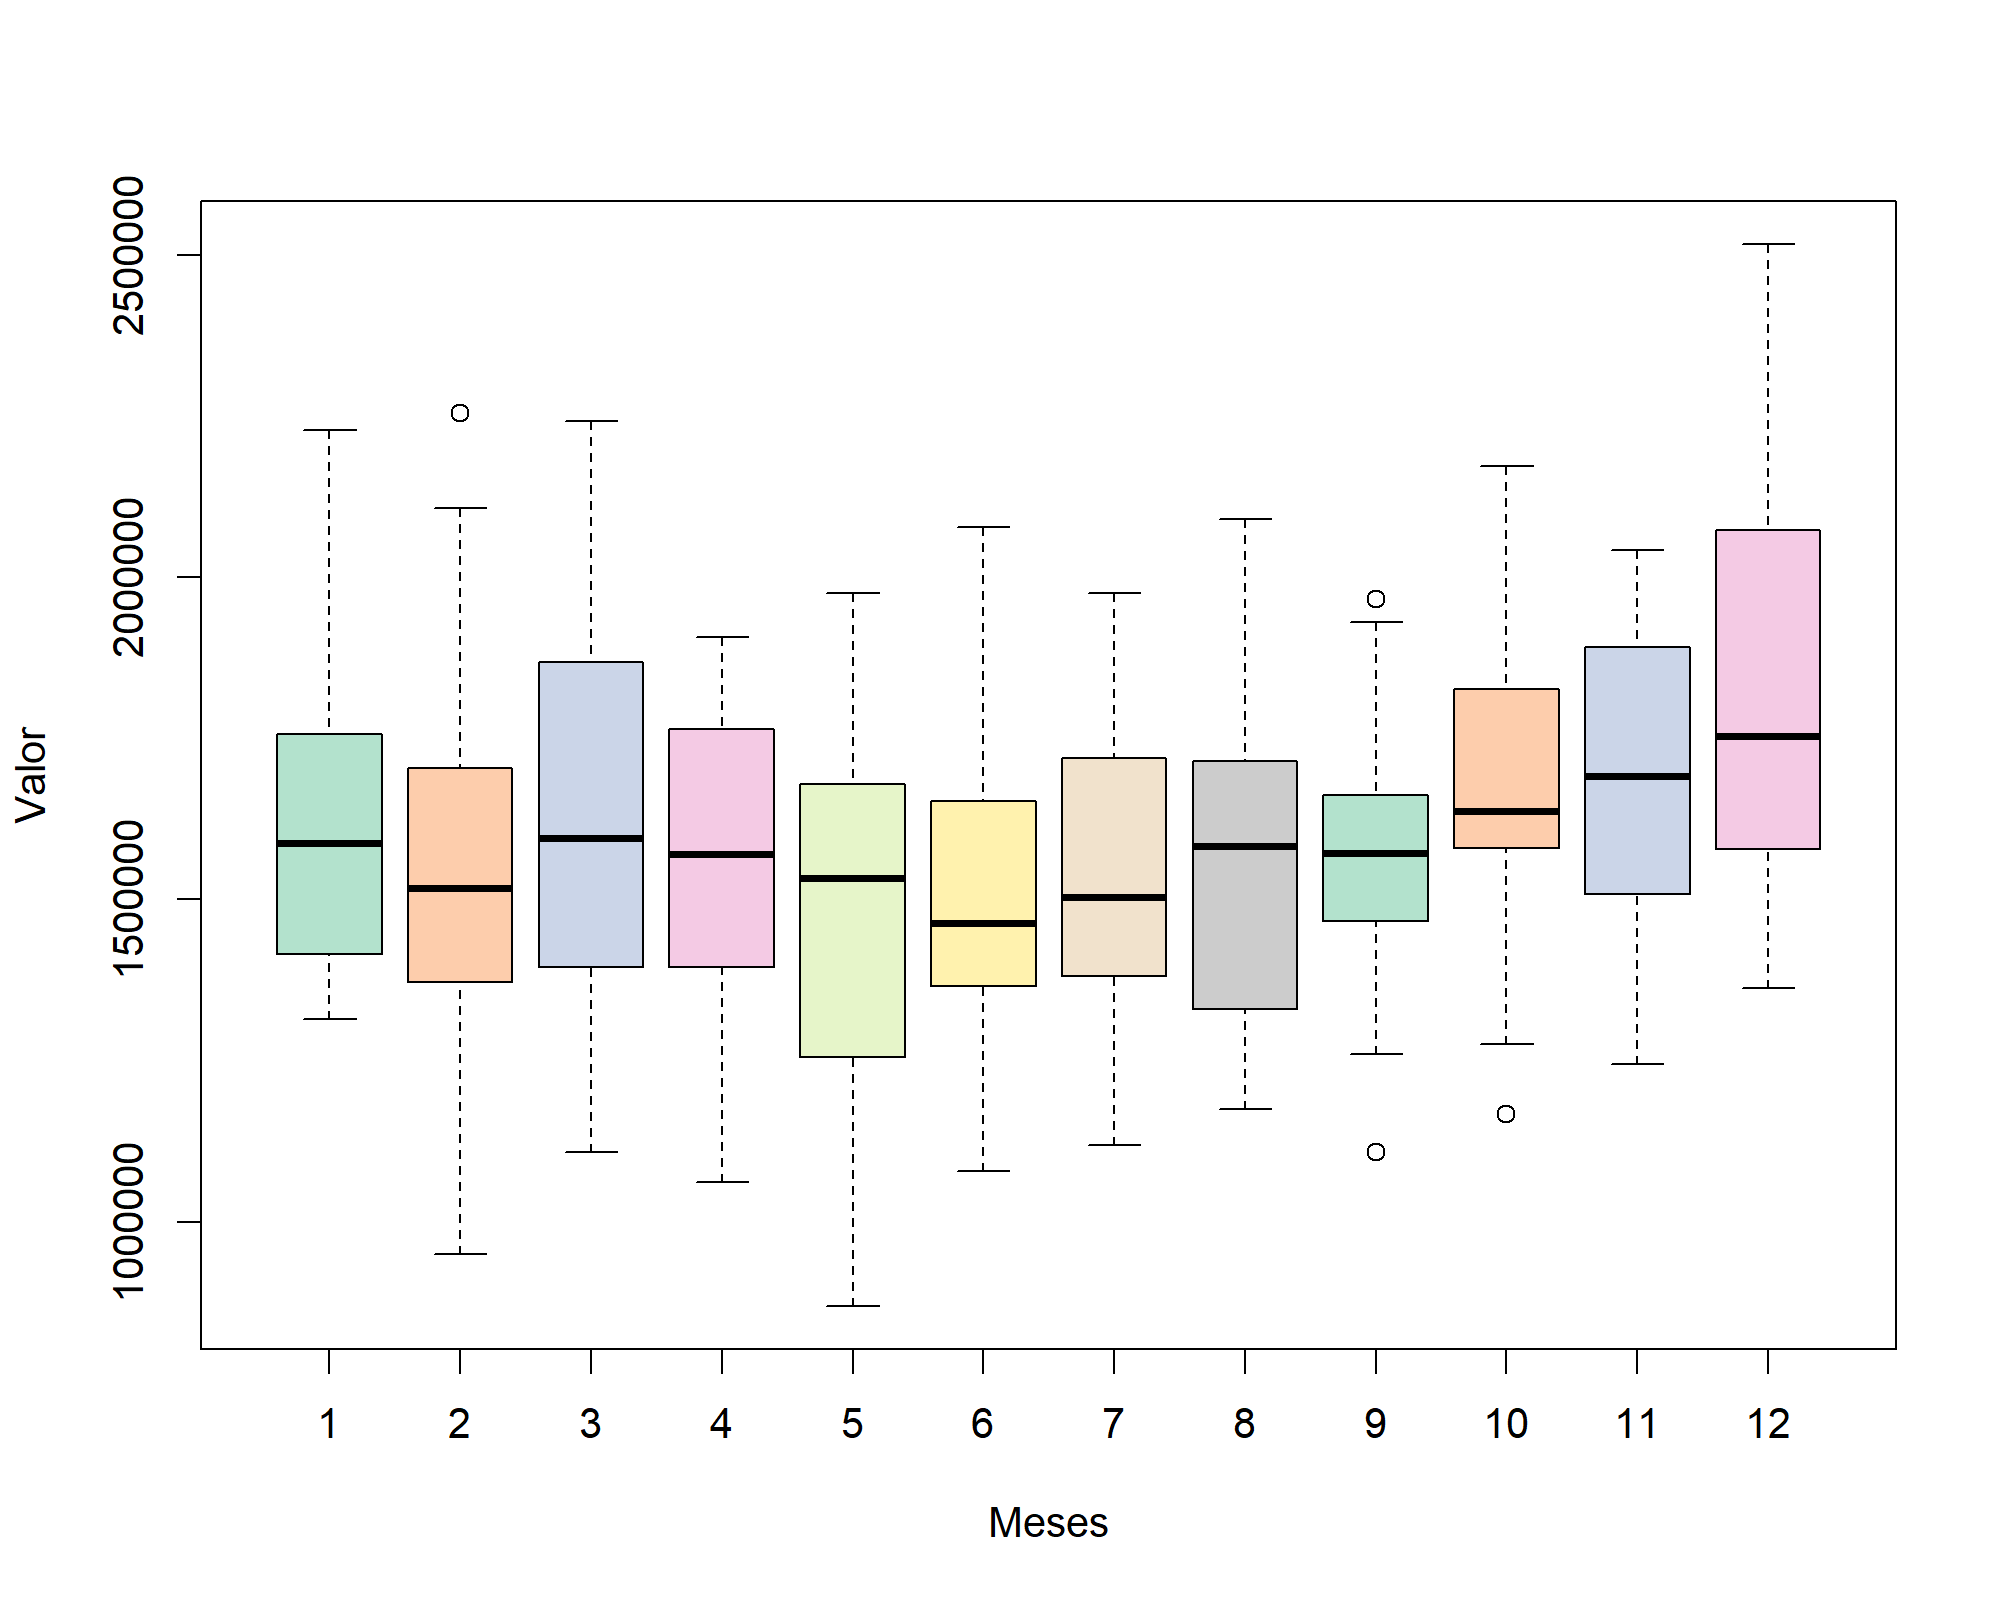
\includegraphics[scale=0.8]{boxplot2.png}
\caption{Diagrama de caja y bigotes del valor de producción del tipo de obra Agua, riego y saneamiento por meses.}
\label{fig:fig2}
\end{figure}
\end{center}

\begin{center}
\begin{figure}[H]
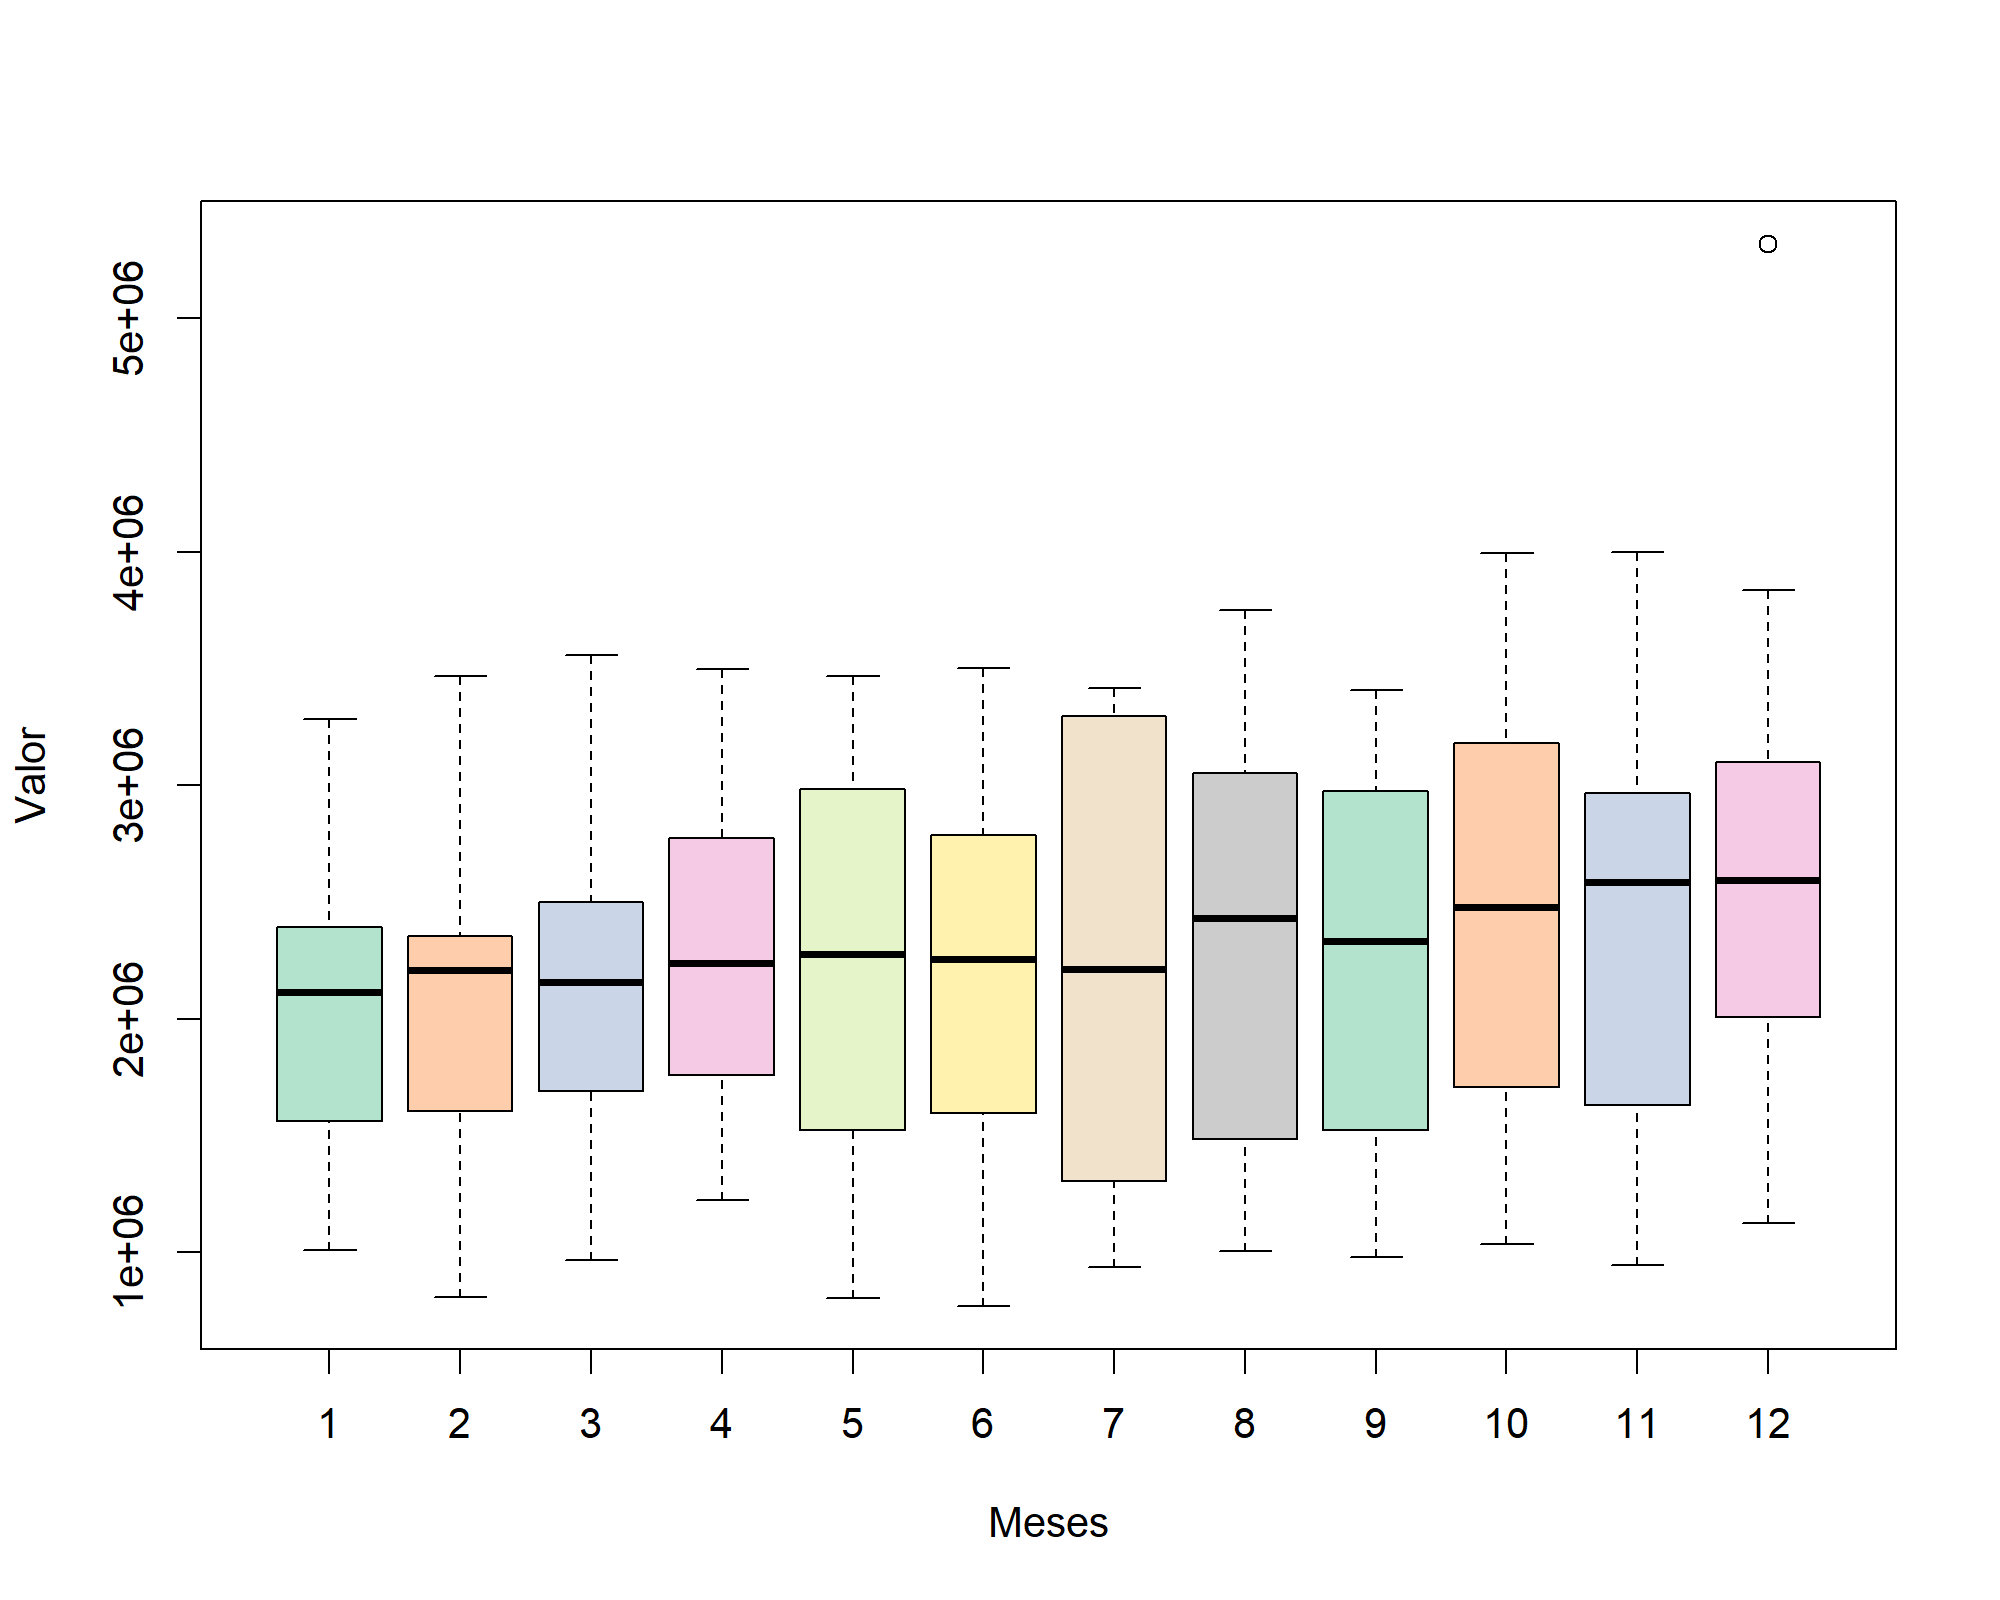
\includegraphics[scale=0.8]{boxplot3.png}
\caption{Diagrama de caja y bigotes del valor de producción del tipo de obra Electricidad y comunicaciones por meses.}
\label{fig:fig3}
\end{figure}
\end{center}

\begin{center}
\begin{figure}[H]
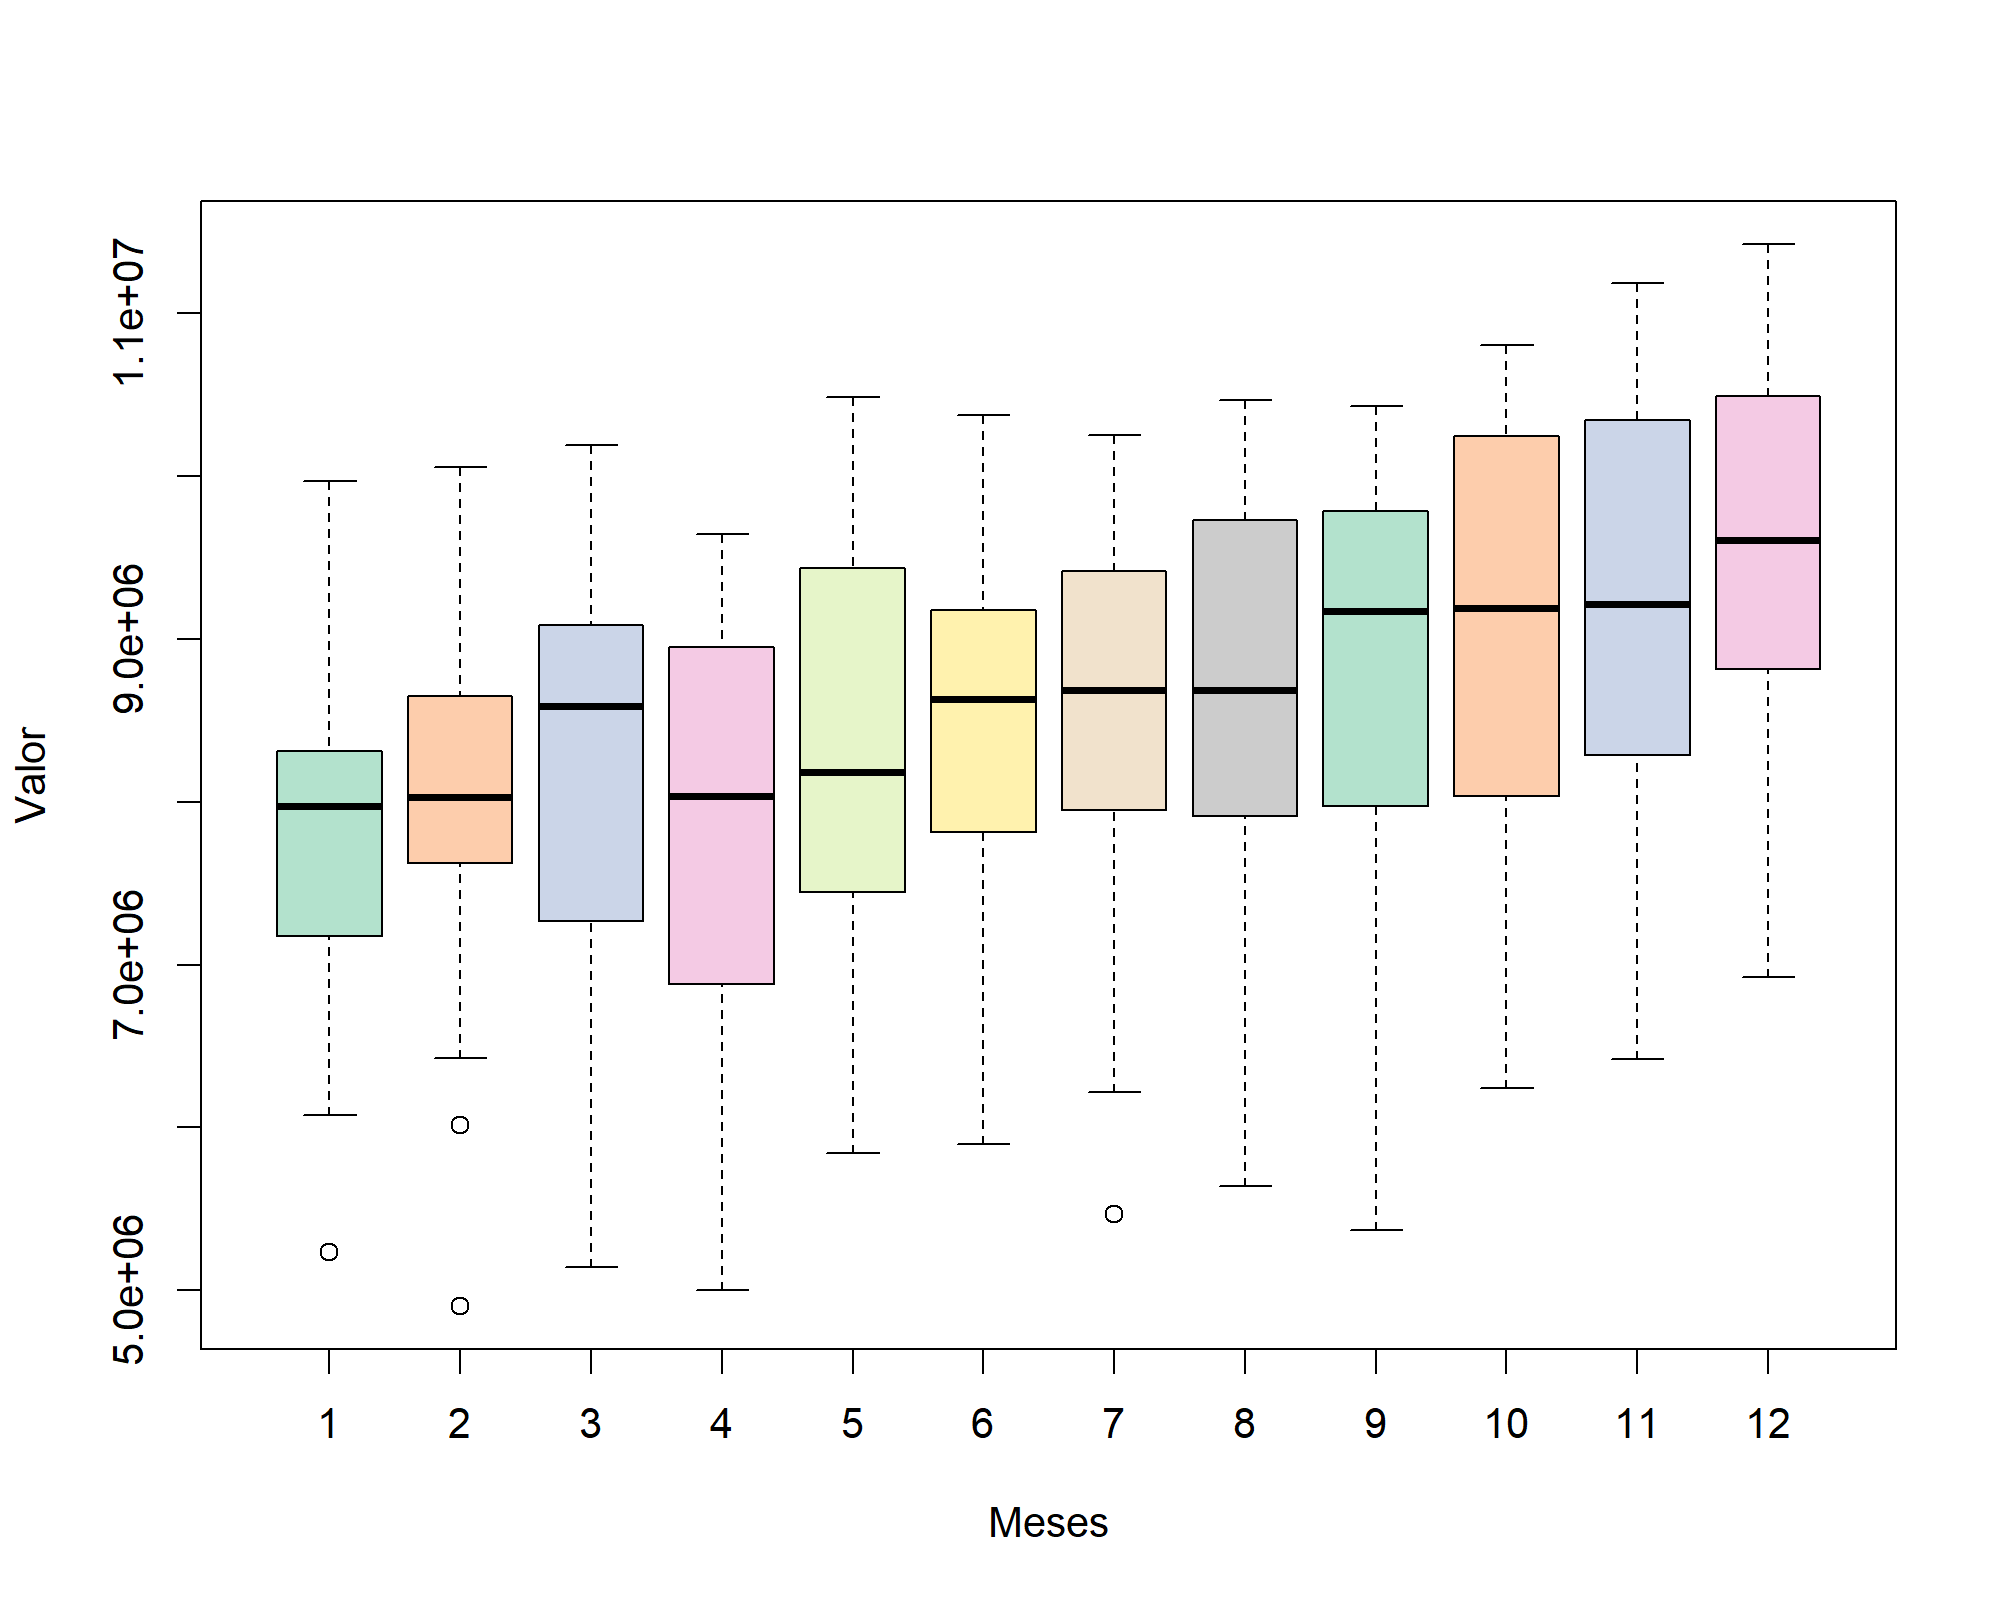
\includegraphics[scale=0.8]{boxplot4.png}
\caption{Diagrama de caja y bigotes del valor de producción del tipo de obra Transporte por meses.}
\label{fig:fig4}
\end{figure}
\end{center}

\begin{center}
\begin{figure}[H]
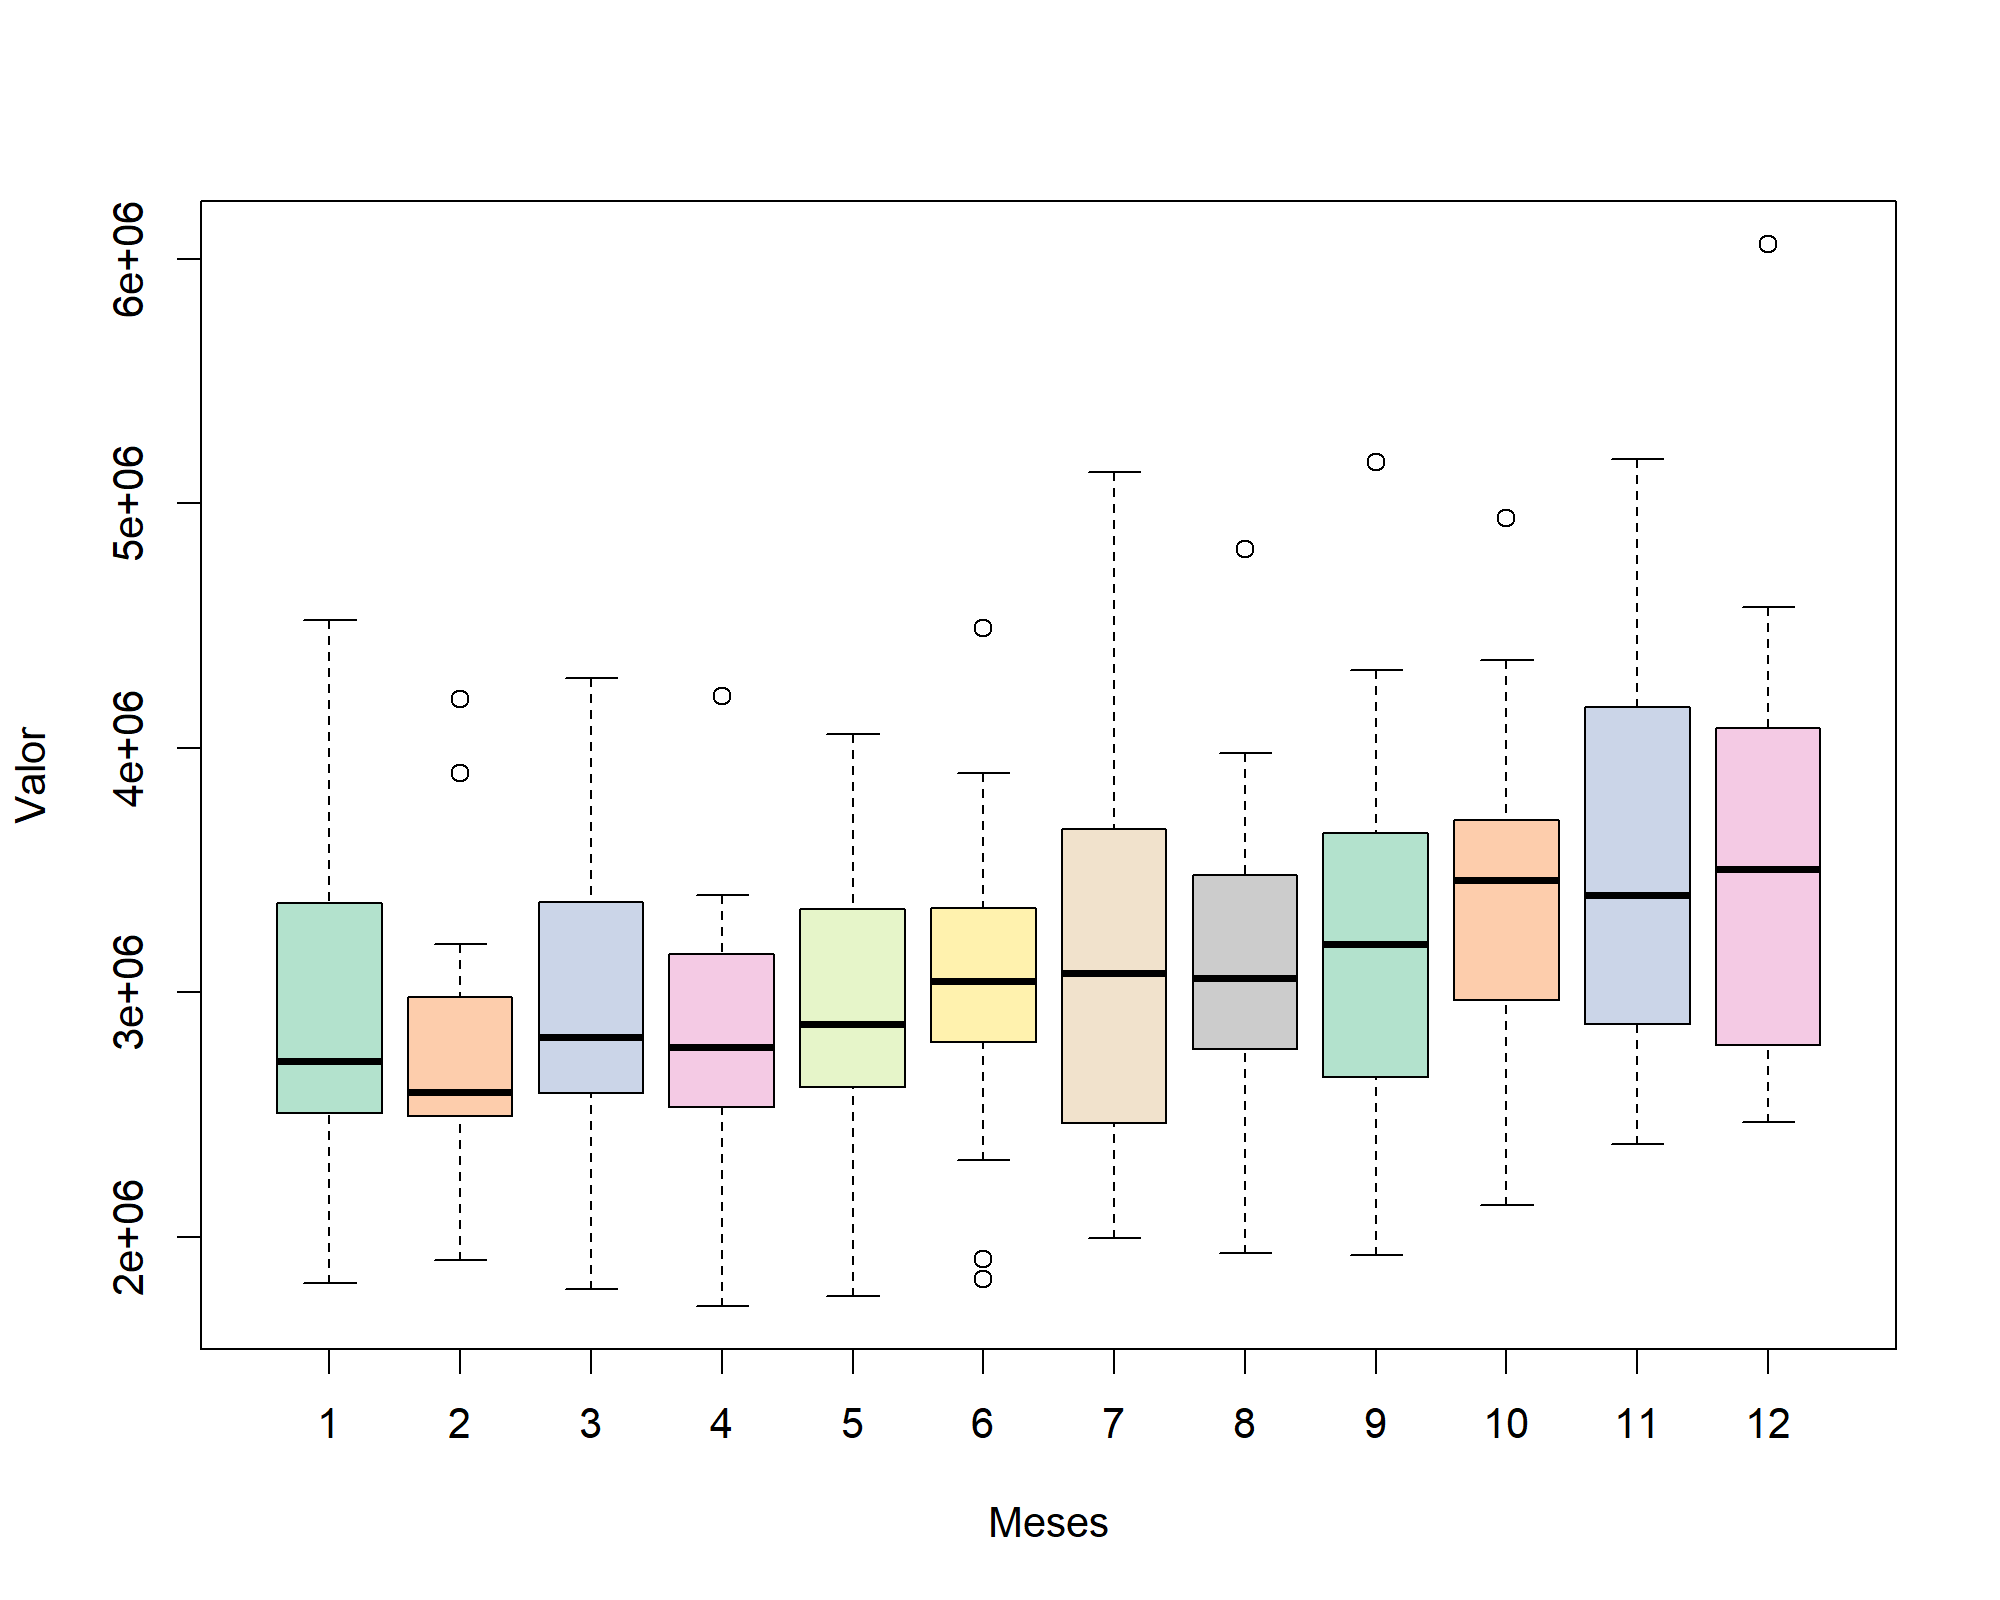
\includegraphics[scale=0.8]{boxplot5.png}
\caption{Diagrama de caja y bigotes del valor de producción del tipo de obra Petróleo y petroquímica por meses.}
\label{fig:fig5}
\end{figure}
\end{center}

\begin{center}
\begin{figure}[H]
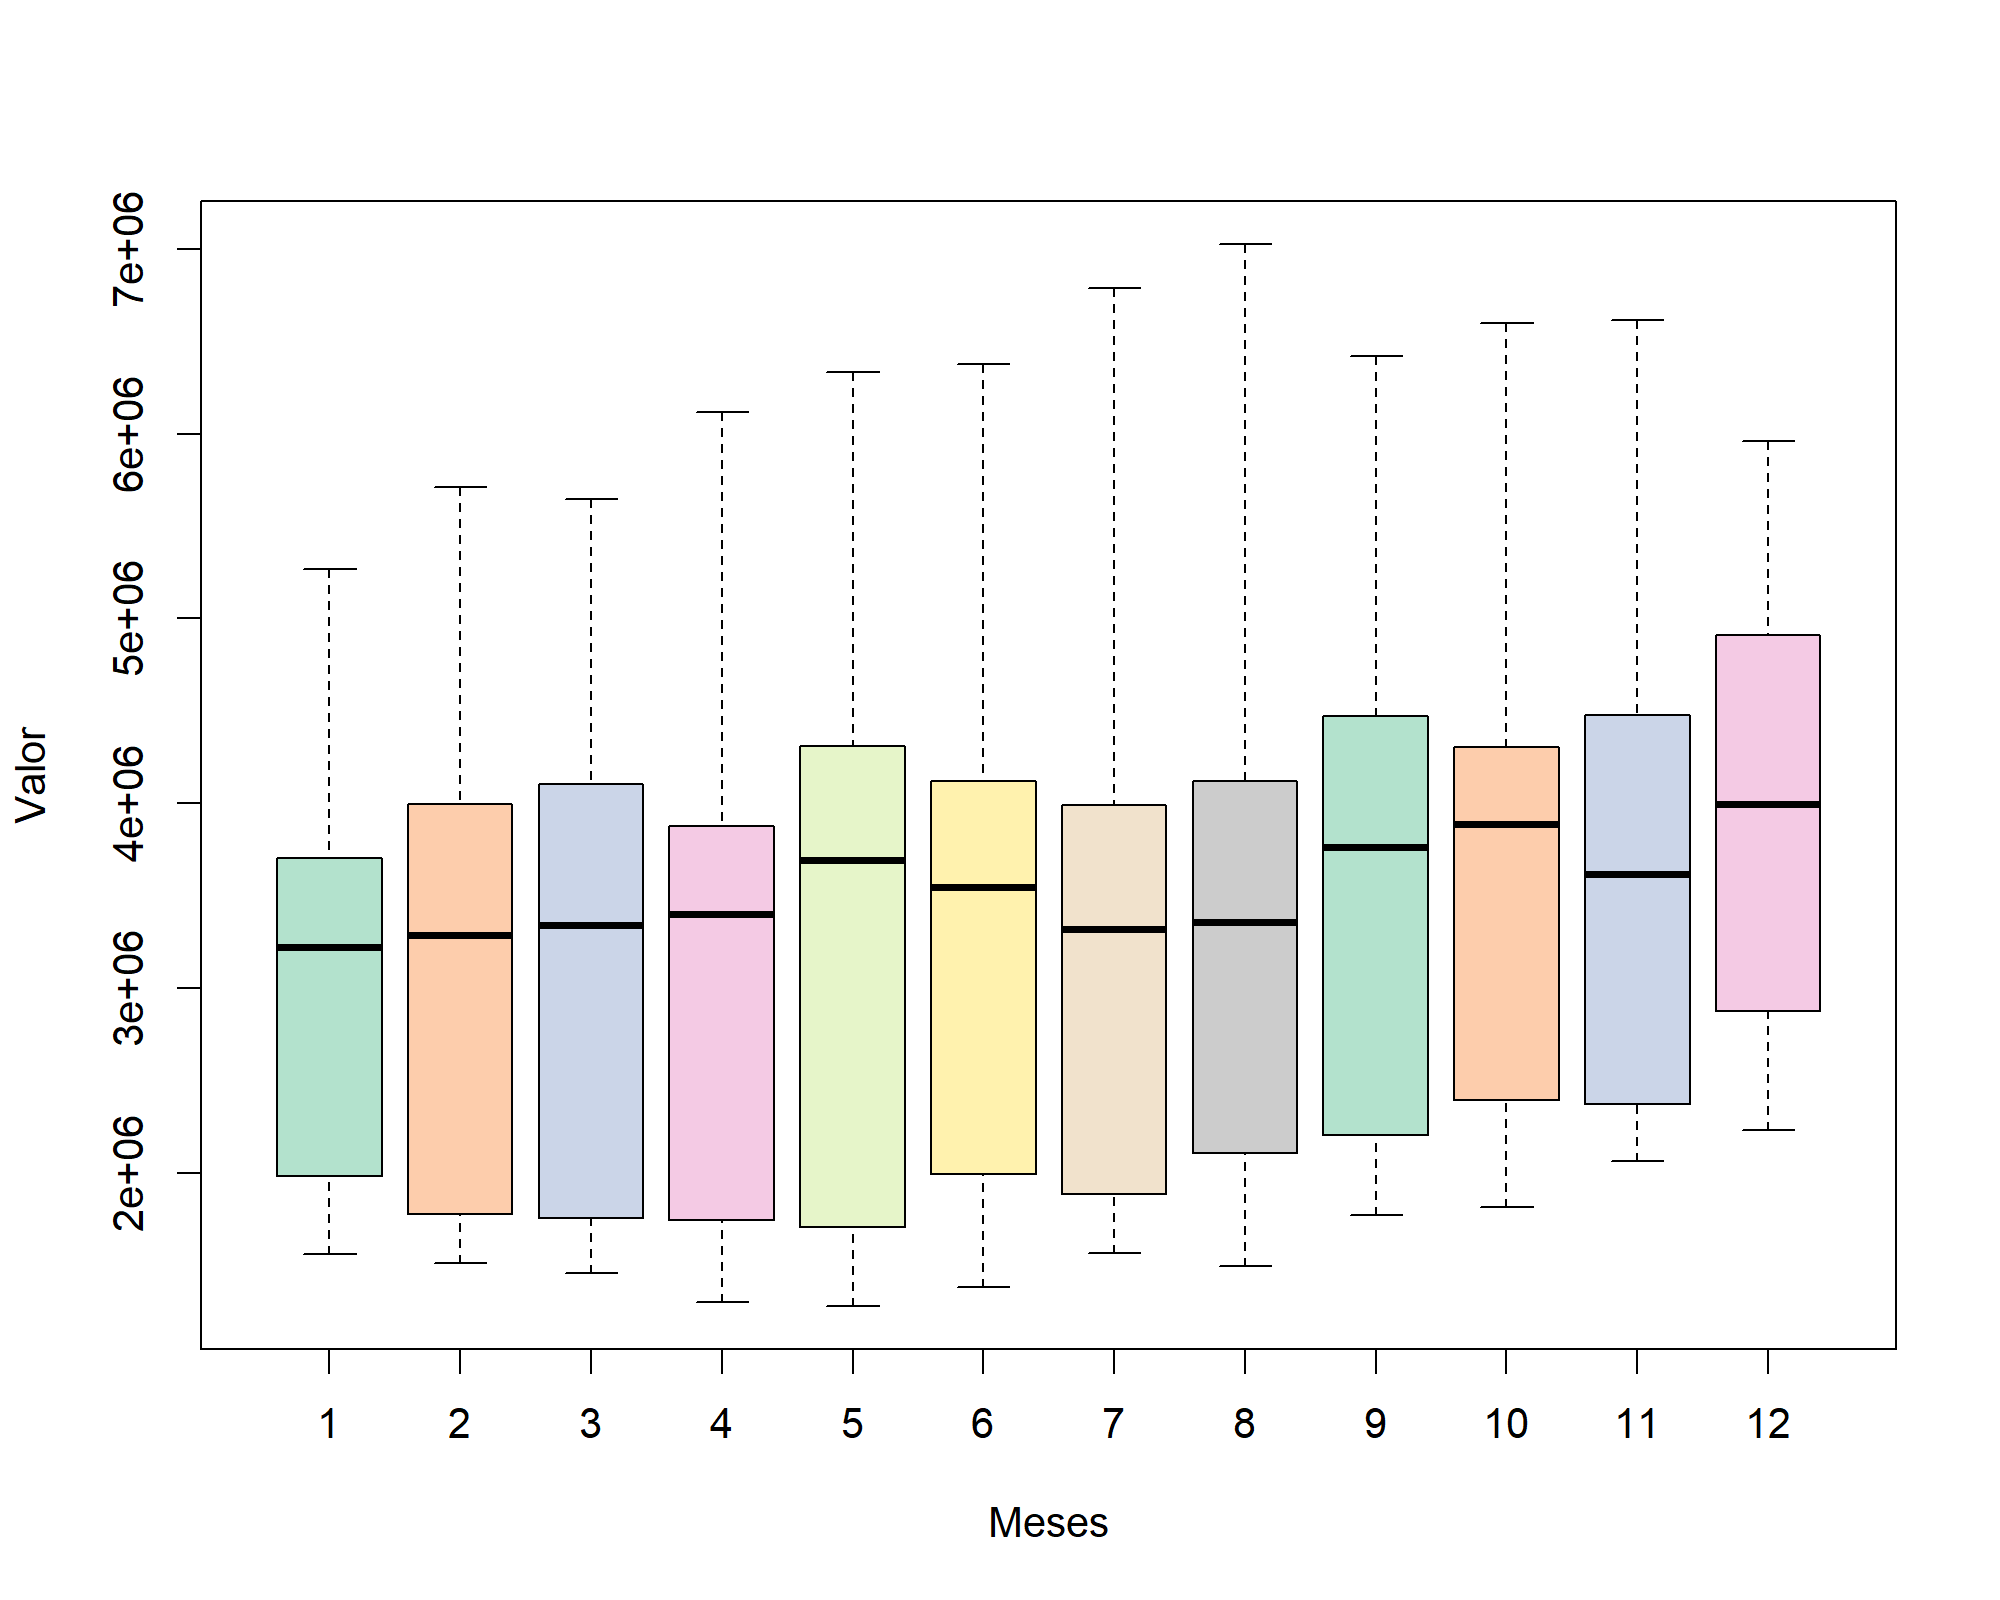
\includegraphics[scale=0.8]{boxplot6.png}
\vspace{-0.6cm}
\caption{Diagrama de caja y bigotes del valor de producción del tipo de obra Otras obras por meses.}
\label{fig:fig6}
\end{figure}
\end{center}
\vspace{-1.4cm}
Para la realización del resumen y las gráficas se elaboró un el código de R \ref{cod:2} de la página \pageref{cod:2}, el código general se encuentra disponible en el repositorio \href{https://github.com/Albertomnoa/Tareas_MPA/Tarea1}{https://github.com/Albertomnoa/Tareas\_MPA} 

\begin{center}
\lstinputlisting[language=R, firstline=16, lastline=31]{Graficar.R}
\label{cod:2}
\end{center}

\section{Conclusiones}
 \begin{itemize}
     \item El tipo de obra con mayor valor de producción es la de Edificaciones y las de menor valor son Agua, riego y saneamiento y Electricidad y comunicaciones.
     \item A partir de los años 2016 y 20017 el tipo de obra Petróleo y petroquímicas bajo su valor de producción con respecto al sector Electricidad y comunicaciones. 
     \item El valor de todos los tipos de obras presentan una caída a partir del año 2019 con respecto a la tendencia creciente de las mismas hasta el 20018.
     \item Los meses donde mayores valores de producción se reportaron fue en los del ultimo trimestre de cada año.
 \end{itemize}

\newpage
\bibliographystyle{plain}
\bibliography{tarea1}

\end{document}
